\vspace*{-5mm}
\mysection{Implementation, Integration \& Test Plan}
In this section we will show the plan we have projected for implementing EasyLib. We will describe the strategy for the processes chosen for approaching the project and the structure of our team, how it is divided and the tasks that each part has to accomplish. After we will state how each team’s part has to interact with the others and the span of time of these interactions. Finally, we will supply a list of possible risks, the probability of their presence, their impact and a possible strategy to deal with them.

\mysubsection{Strategy adopted}
To give a quality assurance of the project and to be sure that the final product we have followed an Agile planning process. It consists in a first initiating part in which we have stated an overall plan application that we have implemented. We have defined the EasyLib’s requirements, discussed and stated the flow of each interaction and the specific technology to use. 
After this part, we followed the well know agility’s cycle, composed by the subsequent phases: Executing, monitoring and Controlling, Closing and Planning. Every cycle round has as input a specific process to accomplish, that is divided between the various team’s parts. After the execution of all the tasks in a precise given timeframe, the work were checked by all the parts. When the discussion on the work done has been terminated and an agreement has been reached, another planning phase containing also the corrections agreed. This cycle has been repeated until the end of the project.

\vspace*{0cm}
\begin{figure}[H]
	\centering
	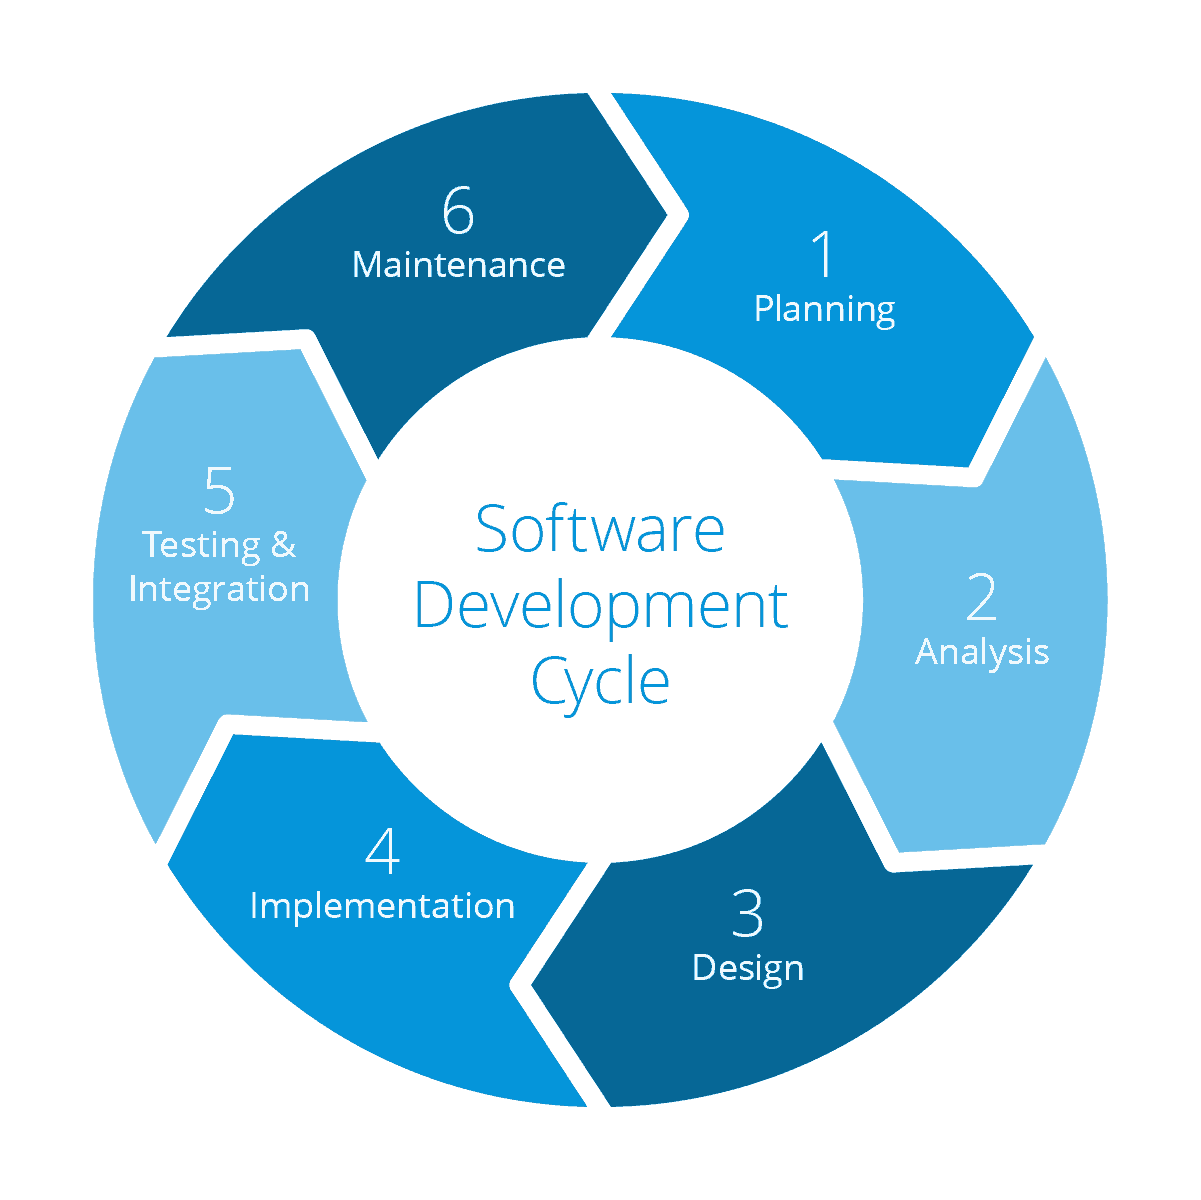
\includegraphics[scale=0.21]{Images/Diagrams/agility_cycle}
	\caption{Agility cycle}
\end{figure}

\mysubsection{Team Structure}
Our team is composed by two Computer engineers with complementary competences and that have dealt with different tasks throughout the development process. The main tasks performed are that one listed and commented right below.

\begin{itemize}
\item \emph{Client Front-End development:}this role required the full understanding of the android components related to the visualization part, the high level of image-editing software in order to produce the aimed layout and the management of the application server requests and the arrangement of the information contained in the responses to produce the whished view result. 

\item \emph{Client Back-End and Application Server development:} this role required a deep knowledge of how to build asynchronous socket multi-client network infrastructure, a good understanding in multi-table MySQL databases management, including SQL statement and trigger implementation. Nonetheless, this team component has dealt with the Android services and their communication with the application server and the main thread of the app.
\end{itemize}

\mysubsection{Implementation process}
The work has been divided in three milestones. In these spans of time the team members were required to complete the tasks that have been established in the previous planning phase. Every week a meeting to discuss about the progresses were attended and new agreement finalized to proceed at the same speed were taken. If a team’s part terminated his tasks before the milestone’s day, it usually anticipated the work programmed for the subsequent milestone but remaining ready for eventually applying changes or corrections on the software already implemented. After each milestone, some days were employed for integrating front-end and back-end part to have always a working prototype. \\
At the end of the implementation process the team has performed a Unit testing and functional testing campaign, in order to assure that all the functionalities worked correctly. Also a User acceptance test have been carried on, involving a restrict group of people which gave back feedback on their user experience that drove the developing process.

